\documentclass[../main/main.tex]{subfiles}

%_______________________________________________________________________________________________________________________
\begin{document}




\section{Paralelismo}




%-------Slide 1-------	
%----------------------------------------------------------------------------------------------------------------------	
\setLayout{mainpoint}
\begin{frame}
	\frametitle{Paralelismo}
\end{frame}
%----------------------------------------------------------------------------------------------------------------------	



%-------Slide 2-------	
%----------------------------------------------------------------------------------------------------------------------	
\setLayout{vertical}
\begin{frame}{\smaller \smaller Tecnologias Empregadas}
	\vspace{-0.25cm}
	\smaller
	\begin{block}{\smaller MPI}
		MPI (Message Passing Interface) é um padrão de comunicação amplamente utilizado em computação paralela e distribuída. Ela define um conjunto de rotinas e funções que permitem a troca de mensagens entre processos que podem estar executando em diferentes nós de um cluster ou em diferentes núcleos de um mesmo computador(\url{https://www.open-mpi.org/}).
	\end{block}
	\begin{block}{\smaller Zoltan}
		A biblioteca Zoltan, desenvolvida pelo Sandia National Laboratories, é um kit de ferramentas de software projetado para simplificar o desenvolvimento e otimizar o desempenho de aplicações paralelas, especialmente aquelas que lidam com dados não estruturados e adaptativos. Seu foco principal é fornecer serviços de gerenciamento de dados, com destaque para o balanceamento de carga dinâmico, uma tarefa crucial para garantir a eficiência de computadores paralelos (\url{https://sandialabs.github.io/Zoltan/}).
	\end{block}
	\begin{block}{\smaller boost/geometry}
		É uma biblioteca da coleção \textbf{Boost C++ Libraries} voltada para o processamento geométrico genérico. Ela fornece um conjunto abrangente de ferramentas e algoritmos para manipular e analisar objetos geométricos de forma eficiente, permitindo trabalhar com diferentes tipos de coordenadas e sistemas de referência, mantendo alta flexibilidade e desempenho (\url{https://www.boost.org/}).
	\end{block}
\end{frame}
%----------------------------------------------------------------------------------------------------------------------	




%-------Slide 3-------	
%----------------------------------------------------------------------------------------------------------------------	
\setLayout{vertical}
\begin{frame}
	\begin{block}{}
		O \textit{HigFlow/HigTree}  é executada em paralelo com memória distribuída, utilizando a API \textbf{MPI} para comunicação entre processos.
		O domínio é particionado por meio do algoritmo \textbf{Recursive Coordinate Bisection} (\textbf{RCB}) da biblioteca \textbf{Zoltan}, garantindo balanceamento de carga.
		A comunicação entre fronteiras é tratada com regiões de sobreposição (fringe), definidas pela \textbf{boost/geometry}, assegurando a troca correta de dados entre vizinhos (\citeauthoronline{raymundo}).
	\end{block}
\end{frame}
%----------------------------------------------------------------------------------------------------------------------	



%-------Slide 3-------	
%----------------------------------------------------------------------------------------------------------------------	
\setLayout{vertical}
\begin{frame}[fragile]{\smaller\smaller Algorítimo Recursive Coordinate Bisection}
        \vspace{-0.50cm}
		\fontsize{7}{8}
		\begin{verbatim}
FUNÇÃO RCB(Região, NumPartesDesejadas)
    SE NumPartesDesejadas == 1 ENTÃO
        Retorne Região  // Já atingimos o número desejado de partes
    FIM SE
    
    // 1. Selecionar o eixo de corte
    // Escolha o eixo (X, Y ou Z) que corresponde à dimensão mais longa da caixa delimitadora da região
    Eixo = EscolherEixoMaisLongo(Região)
    
    // 2. Calcular o ponto de corte
    // Encontre o ponto de corte ao longo do eixo selecionado que divide o peso dos dados igualmente
    PontoCorte = CalcularPontoCorte(Região, Eixo)
    
    // 3. Dividir a região
    Região1, Região2 = DividirRegião(Região, Eixo, PontoCorte)
    
    // 4. Dividir recursivamente as sub-regiões
    // Determine como distribuir o número de partes entre as duas sub-regiões
    NumPartesRegião1, NumPartesRegião2 = DistribuirPartes(NumPartesDesejadas)
    
    Resultado1 = RCB(Região1, NumPartesRegião1)
    Resultado2 = RCB(Região2, NumPartesRegião2)
    
    // 5. Combinar os resultados
    Retorne Combinar(Resultado1, Resultado2)
FIM FUNÇÃO
		\end{verbatim}

\end{frame}
%----------------------------------------------------------------------------------------------------------------------	



%-------Slide 4-------	
%----------------------------------------------------------------------------------------------------------------------	
\setLayout{vertical}
\begin{frame}
        \vspace{1cm}
        \centering
    	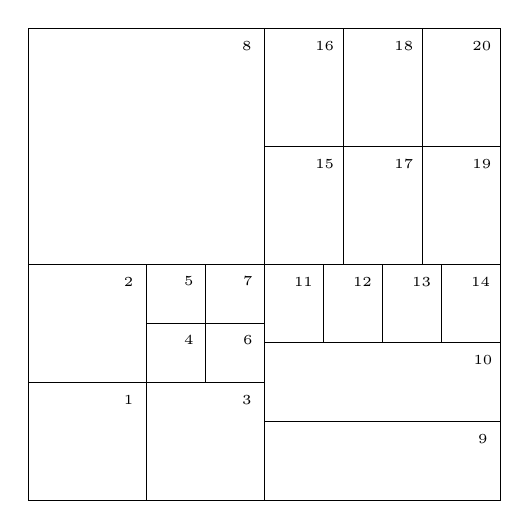
\begin{tikzpicture}[scale=1.5]
        
        \draw (0,0) rectangle (4,4);
        \draw (2,2) rectangle (4,4);
        \draw (0,0) rectangle (2,2);
        
        \draw (0,0) rectangle (1,1);
        \draw (0,1) rectangle (1,2);
        \draw (1,0) rectangle (2,1);
        \draw (1,1) rectangle (1.5,1.5);
        \draw (1.5,1.5) rectangle (2,2);
        
        \draw (2,2) rectangle (2.67,3);
        \draw (2.67,2) rectangle (3.34,3);
        \draw (3.34,2) rectangle (4,3);
        
        \draw (2,3) rectangle (2.67,4);
        \draw (2.67,3) rectangle (3.34,4);
        \draw (3.34,3) rectangle (4,4);
        
        \draw (2,0) rectangle (4,0.67);
        \draw (2,0.67) rectangle (4,1.34);
        \draw (2,1.34) rectangle (2.5,2);
        \draw (2.5,1.34) rectangle (3,2);
        \draw (3,1.34) rectangle (3.5,2);
        
        % Numerando os retângulos
        \node at (0.85,0.85) {\tiny 1};
        \node at (0.85,1.85) {\tiny 2};
        \node at (1.85,0.85) {\tiny 3};
        \node at (1.36,1.36) {\tiny 4};
        \node at (1.36,1.86) {\tiny 5};
        \node at (1.86,1.36) {\tiny 6};
        \node at (1.86,1.86) {\tiny 7};
        \node at (1.85,3.85) {\tiny 8};
        \node at (3.85,0.52) {\tiny 9};
        \node at (3.85,1.19) {\tiny 10};
        \node at (2.33,1.85) {\tiny 11};
        \node at (2.83,1.85) {\tiny 12};
        \node at (3.33,1.85) {\tiny 13};
        \node at (3.83,1.85) {\tiny 14};
        \node at (2.51,2.85) {\tiny 15};
        \node at (2.51,3.85) {\tiny 16};
        \node at (3.18,2.85) {\tiny 17};
        \node at (3.18,3.85) {\tiny 18};
        \node at (3.84,2.85) {\tiny 19};
        \node at (3.84,3.85) {\tiny 20};
        
    \end{tikzpicture}
    \captionof{figure}{Exemplo de malha 2D e sua \textit{quadtree} associada. \\ Fonte: \citeauthoronline{Sousa2019}}
\end{frame}
%----------------------------------------------------------------------------------------------------------------------



%-------Slide 5-------	
%----------------------------------------------------------------------------------------------------------------------	
\setLayout{vertical}
\begin{frame}
    \begin{figure}
        \vspace{1cm}
        \centering
        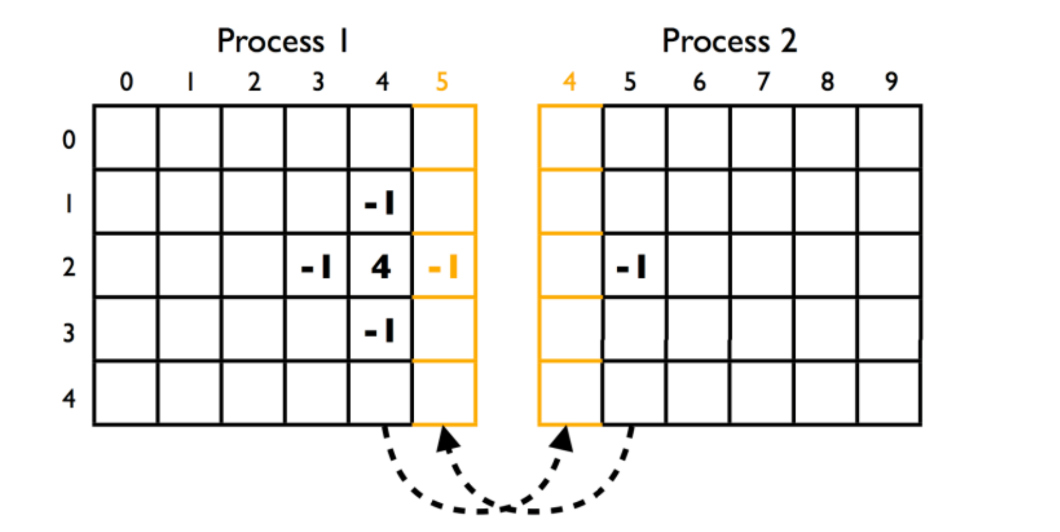
\includegraphics[height=0.6\textheight]{imgs/fringe.png}
        \caption{Exemplo visual de troca de informações em regiões fringe com stencil de laplaciano bidimensional. \\ \centering fonte: \citeauthoronline{raymundo} (\citeyear{raymundo})}
    \end{figure}
\end{frame}
%----------------------------------------------------------------------------------------------------------------------	



%-------Slide 3-------	
%----------------------------------------------------------------------------------------------------------------------	
%----------------------------------------------------------------------------------------------------------------------	



%-------Slide 3-------	
%----------------------------------------------------------------------------------------------------------------------	
%----------------------------------------------------------------------------------------------------------------------	



%-------Slide 3-------	
%----------------------------------------------------------------------------------------------------------------------	
%----------------------------------------------------------------------------------------------------------------------	




\end{document}
%_______________________________________________________________________________________________________________________
